\chapter*{Introducción}\label{chapter:introduction}
\addcontentsline{toc}{chapter}{Introducción}

Para elaborar la junta directiva de una organizaci\'on o proceso se suele usar un sistema electoral en el que el poder de voto puede ser transferido \citep{proxy-vote}.   A ese tipo de elecci\'on se le denomina \textbf{votaci\'on representativa}.   Esta es empleada, por ejemplo, en la confecci\'on de los Comit\'es de Mercado Financiero que regulan el Mercado de Deuda P\'ublica cubano. 

En un sistema de votaci\'on representativa  los votos se transfieren, esto es, si una persona $A$ vota por una persona $B$ y esta, a su vez, vota por  $C$, entonces el voto de $A$ se transfiere a $C$. Luego, cada participante puede ser a la vez votante y candidato. Formalmente, el c\'alculo de los votos obtenidos por un candidato puede ser definido recursivamente de la siguiente manera:
\begin{equation}\label{eq:votes-count}
    \#_{votos}(y) = \begin{cases}
        |V_y| + \underset{x \in V_y}{\sum} \#_{votos}(x) & \text{si } V_y \neq \emptyset \\
        0 & \text{si } V_y = \emptyset 
    \end{cases}
\end{equation}
donde $V_y$ es el conjunto de personas que votaron directamente por $y$. Cada individuo puede votar directamente a lo sumo una vez por otra persona. 

La figura~\ref{fig:r-voting} ilustra un ejemplo de votación en el que $A$ votó por $B$, $B$ y $E$ votaron por $C$ y $C$ votó por $D$. $B$ obtiene solamente el voto de $A$, mientras que $C$ obtiene los votos de $A$, $B$ y $E$. $D$ recibe el voto directo de $C$ y, con este,  los votos indirectos de los restantes participantes. Cerca de cada flecha se encuentra un n\'umero que indica la cantidad de votos que se transfieren. Encima de cada candidato se encuentra el n\'umero de votos que obtiene.

\begin{figure}[h!]
    \centering
    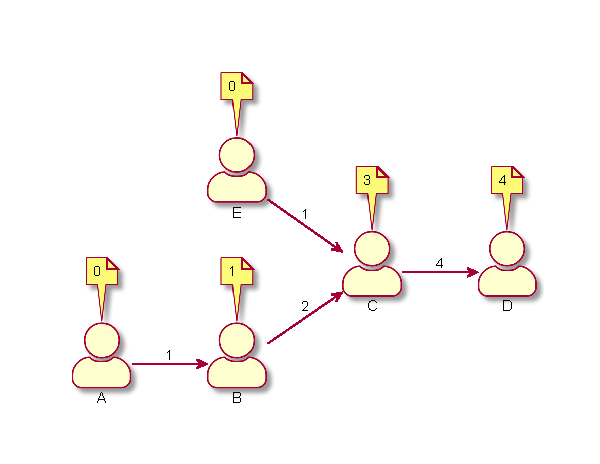
\includegraphics{Graphics/rep-voting.pdf}
    \caption{Conteo de votos en votación representativa.}
    \label{fig:r-voting}
\end{figure}

\todo[disable,inline]{@FIXME ba'jales la altura al pdf generado de las figuras~\ref{fig:r-voting}~y~\ref{fig:voting-cycle}}


En un proceso electoral de este tipo pueden surgir ciclos de votación, como el que se muestra en la figura~\ref{fig:voting-cycle}, donde el voto emitido por $D$ hacia $B$ forma un ciclo que los involucra a ambos y a $C$.  

\begin{figure}[h!]
    \centering
    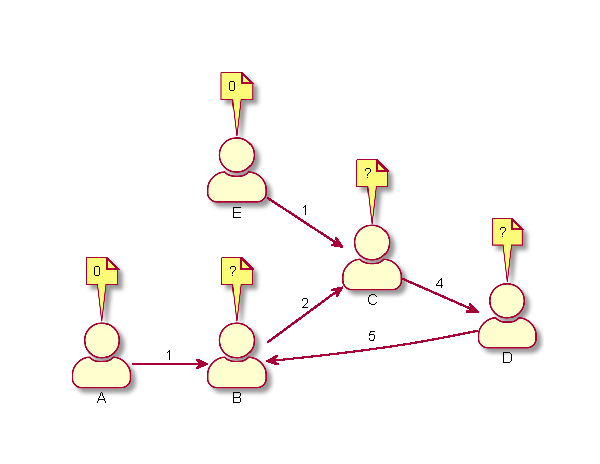
\includegraphics{Graphics/voting-cycle.pdf}
    \caption{Ciclo de votaci\'on.}
    \label{fig:voting-cycle}
\end{figure}


En un  caso como ese, no se puede aplicar sin m\'as la f\'ormula~\eqref{eq:votes-count} para calcular los votos obtenidos por los candidatos involucrados en el ciclo.  La naturaleza recursiva de $\#_{votos}$ impide su c\'alculo en ciclos de votaci\'on, debido a la ocurrencia de dependencias circulares. Por ejemplo, en la figura~\ref{fig:voting-cycle} se puede apreciar que el c\'alculo de los votos que $C$ obtiene depende del c\'alculo de los votos de $B$, y este, a su vez, depende del valor de $\#_{votos}(D)$, pero $D$ depende del n\'umero de votos obtenidos por $C$. Ocurre entonces un c\'irculo de dependencias y no puede ser calculado apropiadamente el n\'umero de votos obtenido por cada uno de los candidatos $B$, $C$ y $D$.



Tradicionalmente en estas elecciones, como en muchas otras, los votos son emitidos en boletas de papel y el conteo es realizado manualmente. Esto puede traer consigo ciertos problemas que causan desconfianza en el electorado, como son los votos falsos y el mal conteo de los votos.   Si no se hace una verificaci\'on rigurosa de la identidad del votante, entonces se puede emitir votos con relativa facilidad en nombre de personas que no han votado (votos falsos). Si el conteo no est\'a supervisado adecuadamente, pueden surgir errores en los resultados, ya sea por intereses personales o errores humanos.

En un sistema de votaci\'on electr\'onico se  pueden lograr diversas formas de verificaci\'on biom\'etrica, por ejemplo, mediante la huella digital o el esc\'aner ocular.  Por otro lado, en estos sistemas se puede contar los votos de manera eficiente mientras se van realizando y se  puede publicar en vivo los resultados.  Otras bondades poseen los sistemas electrónicos, como son la flexibilidad, lo fácil que pueden ser de usar y lo baratos que resultan con respecto a los sistemas tradicionales. 

Se dice que un sistema electrónico de votaci\'on es centralizado cuando depende de que una agencia central se encargue de registrar, manejar, calcular y revisar los votos. Toda la confianza debe entonces ser depositada en esa agencia, lo cual hace vulnerable al sistema \citep{chica2018weaknesses}. Los sistemas descentralizados constituyen una alternativa en ese sentido. Una de las tecnologías descentralizadas empleadas actualmente es \textit{blockchain}.   Se basa en un registro distribuido e inmutable  de transacciones. Lo que se transacciona puede ser tangible, como lo es  una casa o un carro,  o intangible, como el derecho de autor de una obra o el voto de un elector por un candidato (\cite{blockchain-ibm}). La inmutabilidad y seguridad de este registro se basan en principios de  criptografía, descentralizaci\'on y mecanismos de consenso (\cite{blockch-security-ibm}). 


Ethereum es una plataforma \textit{blockchain} que establece una red p\'ublica que ejecuta y verifica c\'odigo de manera segura.   A dicho c\'odigo o al programa que resulta de ejecutarlo se le conoce como contrato inteligente (\cite{eth-aws}). Sobre Ethereum se puede implementar l\'ogica compleja, como  la de un sistema electoral representativo, mediante el uso de contratos inteligentes.  

GoQuorum, tambi\'en conocida como Quorum, es una implementaci\'on de Ethereum capaz de crear redes privadas y con mecanismos de autorizaci\'on. En GoQuorum tambi\'en se puede personalizar el costo del despliegue de los contratos inteligentes, incluso, puede hacerse nulo. Por todo lo dicho anteriormente, GoQuorum es una buena opci\'on en la que implementar un sistema de votaci\'on representativa.


Existen implementaciones de sistemas de votaci\'on en otras \textit{blockchain} (\cite{agora}) y tambi\'en en Ethereum (\cite{ovn} y \cite{borda_count}), pero no se conoce ninguna implementaci\'on de un sistema de voto representativo en GoQuorum.

El \textbf{objetivo general} de este trabajo es dise\~nar algoritmos para el desarrollo de sistemas de votaciones representativas sobre Quorum. Para cumplirlo, se deben lograr los siguientes \textbf{objetivos espec\'ificos}:
\begin{enumerate}
    \item contar los votos correctamente, \label{item:objectives:count}
    \item asignar un n\'umero de votos justo a cada candidato que se encuentra en un ciclo de votaci\'on, \label{item:objectives:cycle}
    \item obtener s\'olo un ganador, \label{item:objectives:winner}
    \item implementar los algoritmos sobre Quorum.
\end{enumerate}

\todo[inline, disable]{@TODO decir que el Instituto de Criptograf\'ia implement\'o un sistema de votaci\'on en hyperledger fabric pero tampoco nos sirve. ?`C\'omo cito eso?}

A continuaci\'on se enumeran las tareas que deben ser realizadas para lograr los objetivos mencionados:
\begin{enumerate}
    \item realizar una revisi\'on de la bibliograf\'ia existente acerca de sistemas de votaci\'on electr\'onico sobre \textit{blockchain}, as\'i como de los sistemas electorales que se utilizan en la actualidad y sus mecanismos de desempate;
    \item valorar los resultados de la revisi\'on anterior;
    \item dise\~nar algoritmos que permitan contar y desempatar apropiadamente;
    \item estudiar el lenguaje de programaci\'on Solidity;
    \item implementar los contratos inteligentes que sean necesarios;
    \item evaluar esos contratos.
\end{enumerate}

% Este documento se estructura de la siguiente forma. En el cap\'itulo~\ref{chapter:state-of-the-art} se realiza una revisi\'on de la literatura existente acerca de sistemas de votaci\'on electr\'onico sobre \textit{blockchain}, as\'i como de los sistemas electorales que se utilizan en la actualidad y sus mecanismos de desempate. En el cap\'itulo~\ref{chapter:design} se dise\~nan los algoritmos que permiten contar y desempatar apropiadamente. En el cap\'itulo~\ref{chapter:implementation} se estudia el lenguaje de programaci\'on Solidity y se implementan los contratos inteligentes que sean necesarios. En el cap\'itulo~\ref{chapter:evaluation} se eval\'uan los contratos inteligentes implementados. Finalmente, en el cap\'itulo~\ref{chapter:conclusions} se presentan las conclusiones y se plantean las futuras investigaciones.

\todo[inline,disable]{@TODO decir d q' va cada capi'tulo. Est\'a arriba comentado}
